% =====================================================================
%  monoT5 Logit Lens on Decoder Cross-Attention
%  Compile with:  pdflatex logit_lens_experiment_report.tex  (run twice)
%  Figure paths are relative to this file (outputs/...), so compile
%  from the 07_monot5_logit_lens/ directory.
% =====================================================================
\documentclass[11pt]{article}

\usepackage[margin=1in]{geometry}
\usepackage{amsmath, amssymb}
\usepackage{graphicx}
\usepackage{booktabs}
\usepackage{longtable}
\usepackage{array}
\usepackage{float}
\usepackage{xcolor}
\usepackage{caption}
\usepackage{enumitem}
\usepackage{listings}
\usepackage[hidelinks]{hyperref}

\definecolor{codegray}{gray}{0.95}
\lstset{
  basicstyle=\ttfamily\footnotesize,
  backgroundcolor=\color{codegray},
  breaklines=true,
  frame=single,
  columns=fullflexible,
  keepspaces=true,
}

\newcommand{\score}{\operatorname{score}}

\title{\textbf{Logit Lens on monoT5 Decoder Cross-Attention \\[2pt]
Under Keyword-Stuffing Adversarial Attacks} \\[6pt]
\large Does the Attack Token Get Directly Promoted, or Only Causally Matter?}
\author{Information-Retrieval Adversarial-Evaluation Project}
\date{\today}

\begin{document}
\maketitle

\begin{abstract}
Experiments~1, 3, and 6 establish that a keyword-stuffing attack's causal
effect on monoT5's relevance score is concentrated in late-layer decoder
cross-attention, a small set of specific attention heads, and (via
query-only positional patching) leaks into the encoder's query
representation. This experiment asks a complementary, more literal
question: if we take each decoder layer's cross-attention contribution —
what it writes into the residual stream — and read it out directly through
the model's own unembedding (a logit lens / direct logit attribution), does
the injected attack token appear \emph{promoted} in the resulting top-k
vocabulary distribution? The answer, checked across all 12 whole-block
layers, 12 Experiment-3-flagged heads, and all 105 attacks, is
\textbf{no}: the attack token's rank in this projection never approaches
the top of the $\sim$32{,}100-token vocabulary in any run type (clean,
control, or attack) — the best rank observed anywhere (any layer, any head,
any run type) is $\approx$1{,}776, and typical ranks are in the
thousands to tens of thousands, essentially unchanged between clean and
attacked inputs at most layers. The top-$k$ tokens themselves are
frequently uninterpretable (non-English word fragments unrelated to the
query, document, or attack vocabulary), and the query/document/attack
bucket composition of top-10 is $\geq$90\% ``other'' at every layer. This
is a genuine, well-supported \textbf{null result for this specific
projection}, not a failure of the attack or of Experiments~1/3/6's causal
findings: Section~\ref{sec:discussion} argues that a single component's
\emph{isolated}, un-renormalised contribution is not expected to encode
target-token identity directly, even when that same component's causal
effect on the final score (measured by patching, as in Experiments~1/3) is
large — the causal effect is mediated through many further layers of
processing that a direct, single-layer read-out cannot see.
\end{abstract}

\tableofcontents
\newpage

% =====================================================================
\section{Introduction and Motivation}
% =====================================================================

Experiments~1, 3, and 6 all establish \emph{causal} claims: patching a
component's activation changes the final score by a measurable amount.
None of them ask what that component's contribution, read out in isolation,
actually \emph{says} — i.e.\ which vocabulary tokens it would favour if the
model's own unembedding were applied to it directly, bypassing every layer
that comes after. This is the classical logit-lens question, and it merges
three closely related analyses that all need the same machinery (capture a
contribution, project it, read off top-$k$):

\begin{enumerate}
  \item \textbf{General logit lens.} Top-5/10/20 tokens and logits at every
  decoder layer's cross-attention contribution, for clean, control, and
  attack inputs.
  \item \textbf{Query/document/attack composition.} Tag each top-10 token
  as attack / query / document / stopword / other; does the attack
  vocabulary come to dominate top-$k$ under attack?
  \item \textbf{Attack-token tracking.} Track the specific injected token's
  rank and logit at every layer, across all three run types, to establish
  whether it is measurably \emph{promoted}.
\end{enumerate}

% =====================================================================
\section{Background and Method}
% =====================================================================

\subsection{Scope: cross-attention only}

Matching Experiments~1 and 3's focus on cross-attention as the locus of the
attack effect (see \texttt{DECISIONS.md} for the full rationale). Whole-block
logit lens runs on all 12 decoder layers, unconditionally; per-head logit
lens is restricted to the 12 \textbf{decoder\_cross\_attn} heads Experiment~3
flagged as important ($\text{combined\_effect\_mean} > 0.02$), read live from
Experiment~3's aggregated output.

\paragraph{Which flagged-head snapshot was used.} This experiment's grid run
was launched while Experiment~3's Grid~A was concurrently being re-run at
$n=100$ (see that report's Section~5); this experiment's flagged-head list
was read \emph{before} that re-aggregation completed, so it reflects
Experiment~3's original $n=10$ snapshot: \texttt{L2-H1, L6-H7, L7-H3, L8-H7,
L9-H2, L9-H11, L11-H0, L11-H2, L11-H3, L11-H6, L11-H8, L11-H11} (12 pairs,
8 distinct head indices). Experiment~3's revised $n=100$ data flags 33
heads overall; a re-run against that list was not performed for this
report — Section~\ref{sec:limits} notes this as a limitation, though
Section~\ref{sec:results}'s null result is strong enough in magnitude that
it is very unlikely a different, larger flagged-head set would overturn it.

\subsection{What gets projected}

At each decoder layer, the cross-attention sublayer's \textbf{contribution}
($\text{out\_hidden} - \text{in\_hidden}$ — what it writes into the residual
stream, not the accumulated hidden state) is projected through
\texttt{model.lm\_head}, scaled by T5's own $d_{\text{model}}^{-0.5}$
convention (\texttt{scale\_decoder\_outputs=True} for this checkpoint),
\textbf{without} re-applying \texttt{final\_layer\_norm}. This is direct
logit attribution of one component, not classical full-residual logit
lens — see \texttt{DECISIONS.md} for why, and
Section~\ref{sec:discussion} for why this choice plausibly explains the
null result below. Per-head contributions are $W_o(\text{zero\_pad}(\text{head
slice}))$ — exact, not approximate, verified by testing that summing all
12 heads' contributions reproduces the whole-block contribution.

\subsection{Tagging and tracking}

Top-10 tokens are tagged \texttt{attack} / \texttt{query} / \texttt{document}
/ \texttt{stopword} / \texttt{other}, attack checked \emph{first} (the
attack-grid words are ordinary English words that can coincidentally
overlap query/document vocabulary — see \texttt{DECISIONS.md}). The
specific attack token (a single SentencePiece token for all 7 words in the
grid, verified) is tracked by rank and raw logit at every layer, for
clean, control, and attack inputs — clean/control give the near-zero
baseline that Section~\ref{sec:results} shows is, in fact, indistinguishable
from the attack run.

% =====================================================================
\section{Experimental Setup}
% =====================================================================

\begin{table}[H]
\centering
\caption{Configuration and scope.}
\begin{tabular}{ll}
\toprule
Parameter & Value \\
\midrule
Model checkpoint & \texttt{castorini/monot5-base-msmarco} (vocab size 32{,}100) \\
$k$ values logged & 5, 10, 20 (all three, not just one) \\
Composition default $k$ & 10 \\
Whole-block scope & all 12 decoder layers \\
Per-head scope & 12 Experiment-3-flagged \texttt{decoder\_cross\_attn} heads \\
Grid run & 105 attacks $\times$ 30 examples \\
Canonical run & \texttt{relevant\_start\_5} $\times$ 100 examples \\
\bottomrule
\end{tabular}
\end{table}

The timing pilot (1 attack, $n=5$, whole-block + 12 flagged heads) measured
$38.0$~s/example on CPU, $\approx$90\% of which is per-head cost (each
flagged head needs its own forward pass with a pre-hook on that layer's
\texttt{.o} projection; whole-block reuses one cached forward pass across
all 12 layers). The full grid (105$\times$30 + 100 canonical =
3{,}250 examples) completed in $\approx$1~hour~10~minutes wall-clock on
1$\times$ L40 GPU, zero failures, zero alignment failures, writing
234{,}106 rows (317~MB total).

% =====================================================================
\section{Results}
\label{sec:results}
% =====================================================================

\subsection{Attack-token tracking: no promotion, at any layer}

\begin{figure}[H]
  \centering
  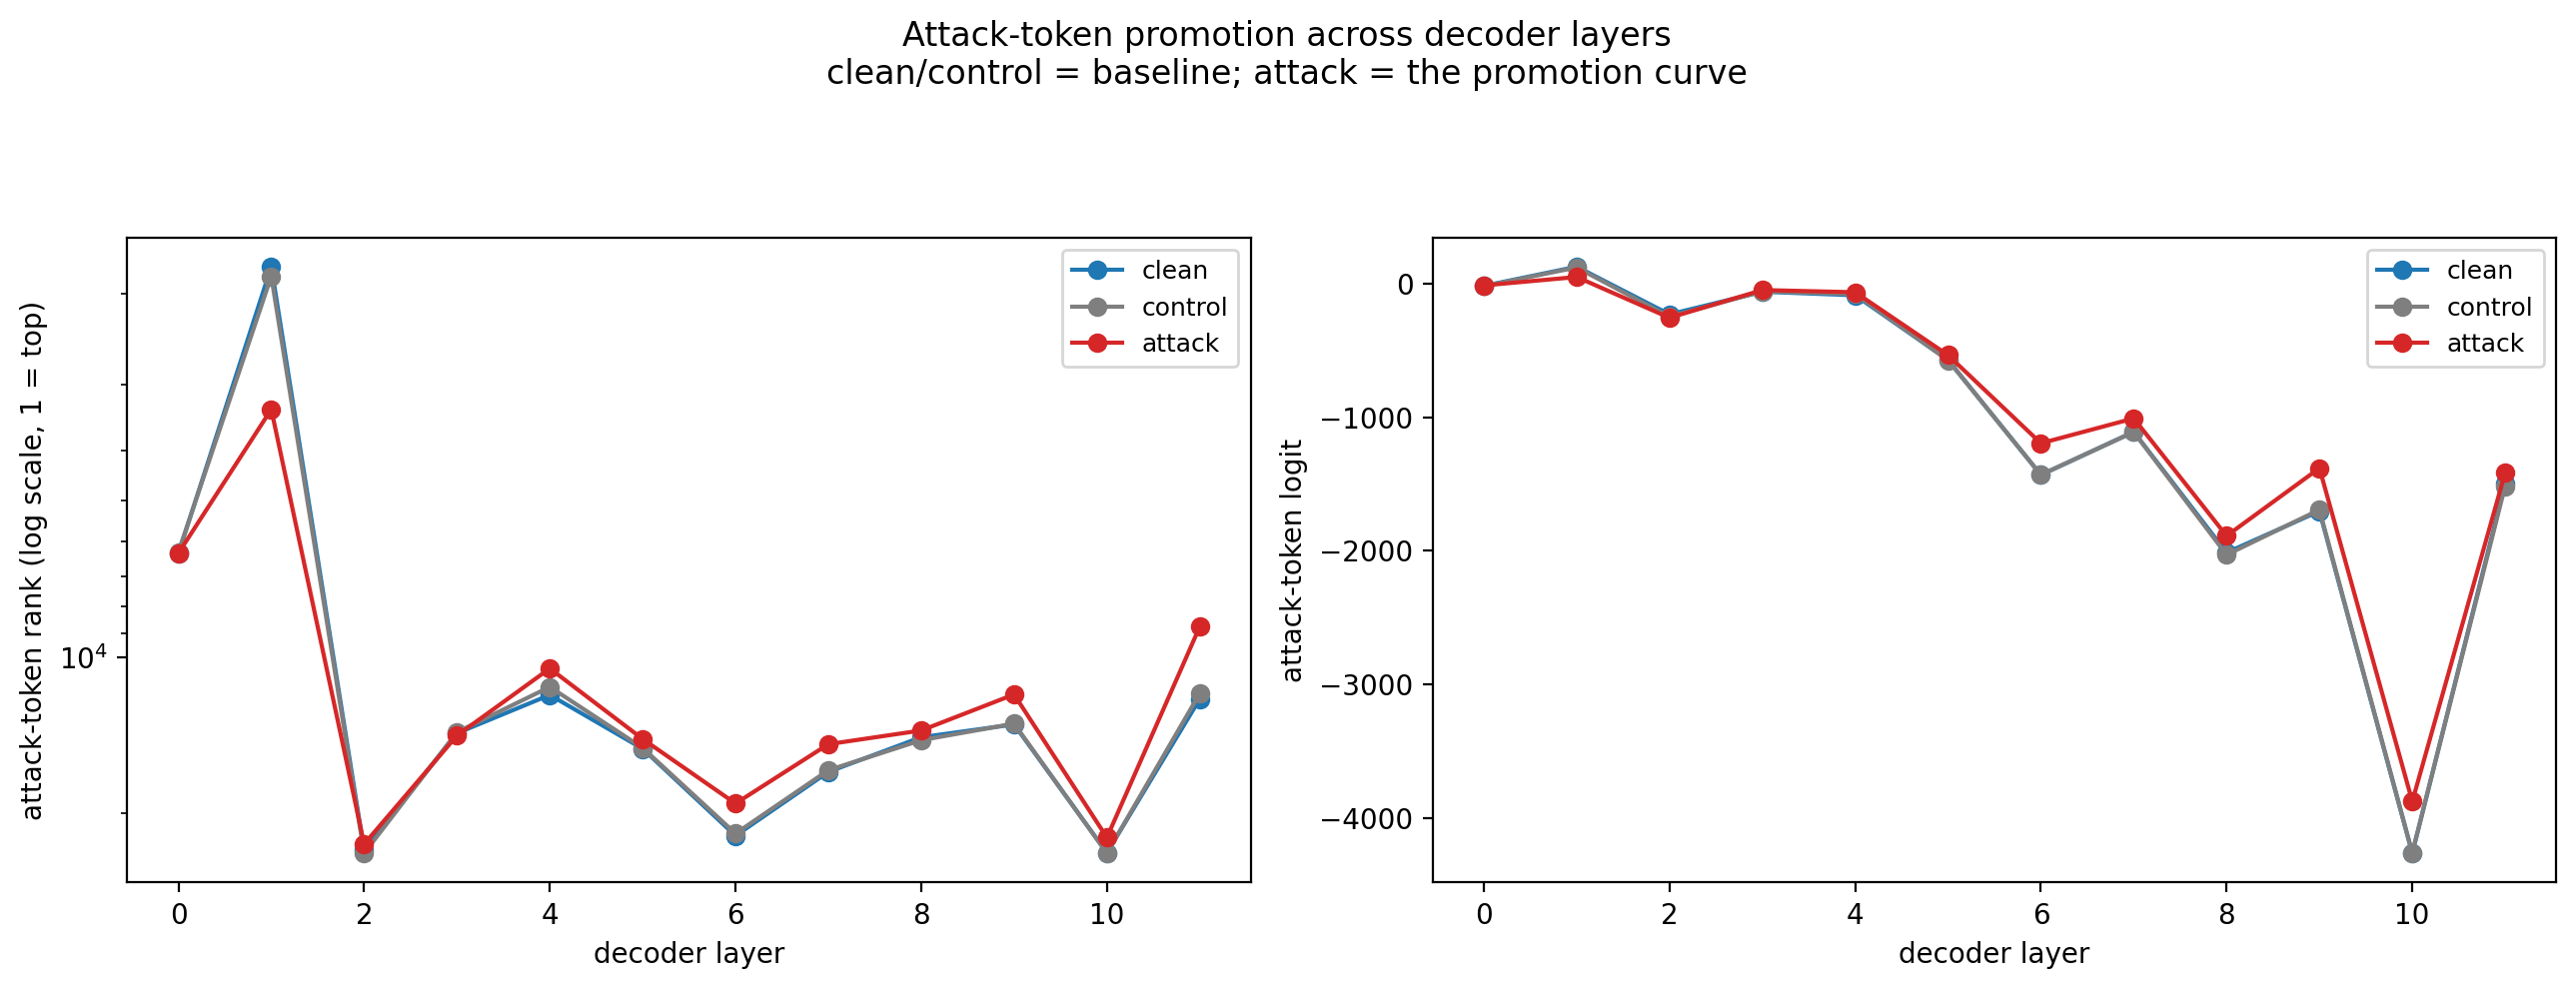
\includegraphics[width=0.95\textwidth]{outputs/plots/attack_token_trajectory.png}
  \caption{Attack-token rank (log scale, 1 = top of vocabulary) and raw
  logit per decoder layer, clean/control/attack overlaid, canonical attack
  ($n=100$).}
  \label{fig:trajectory}
\end{figure}

\begin{table}[H]
\centering
\caption{Attack-token mean rank (out of 32{,}100), whole-block, canonical attack.}
\begin{tabular}{lrrrrrr}
\toprule
Run type & L0 & L1 & L4 & L9 & L10 & L11 \\
\midrule
Clean   & 6{,}322 & 1{,}776 & 11{,}826 & 13{,}474 & 23{,}784 & 12{,}038 \\
Control & 6{,}280 & 1{,}853 & 11{,}413 & 13{,}428 & 23{,}824 & 11{,}746 \\
Attack  & 6{,}313 & 3{,}340 & 10{,}516 & 11{,}799 & 22{,}231 & \phantom{0}8{,}741 \\
\bottomrule
\end{tabular}
\end{table}

The best rank ever observed — any layer, any run type, whole-block or
per-head — is $1{,}776$ (\emph{clean} input, layer~1; not attack). At
layer~1 specifically, the attack run's rank ($3{,}340$) is actually
\emph{worse} than clean's ($1{,}776$). At layer~11, attack's rank
($8{,}741$) is modestly better than clean/control's ($\approx$12{,}000),
the largest directionally-consistent gap observed anywhere in the sweep —
but $8{,}741$ out of $32{,}100$ places the attack token in roughly the
bottom 73\% of the vocabulary by this projection, nowhere close to
top-20. Per-head results do not change this picture: the single best
per-head mean rank across all 12 flagged heads and all 12 layers is
$6{,}472$ (layer~11, head~8) — still three orders of magnitude away from
top-5.

\subsection{Bucket composition: top-10 is $\geq$90\% ``other'' at every layer}

\begin{figure}[H]
  \centering
  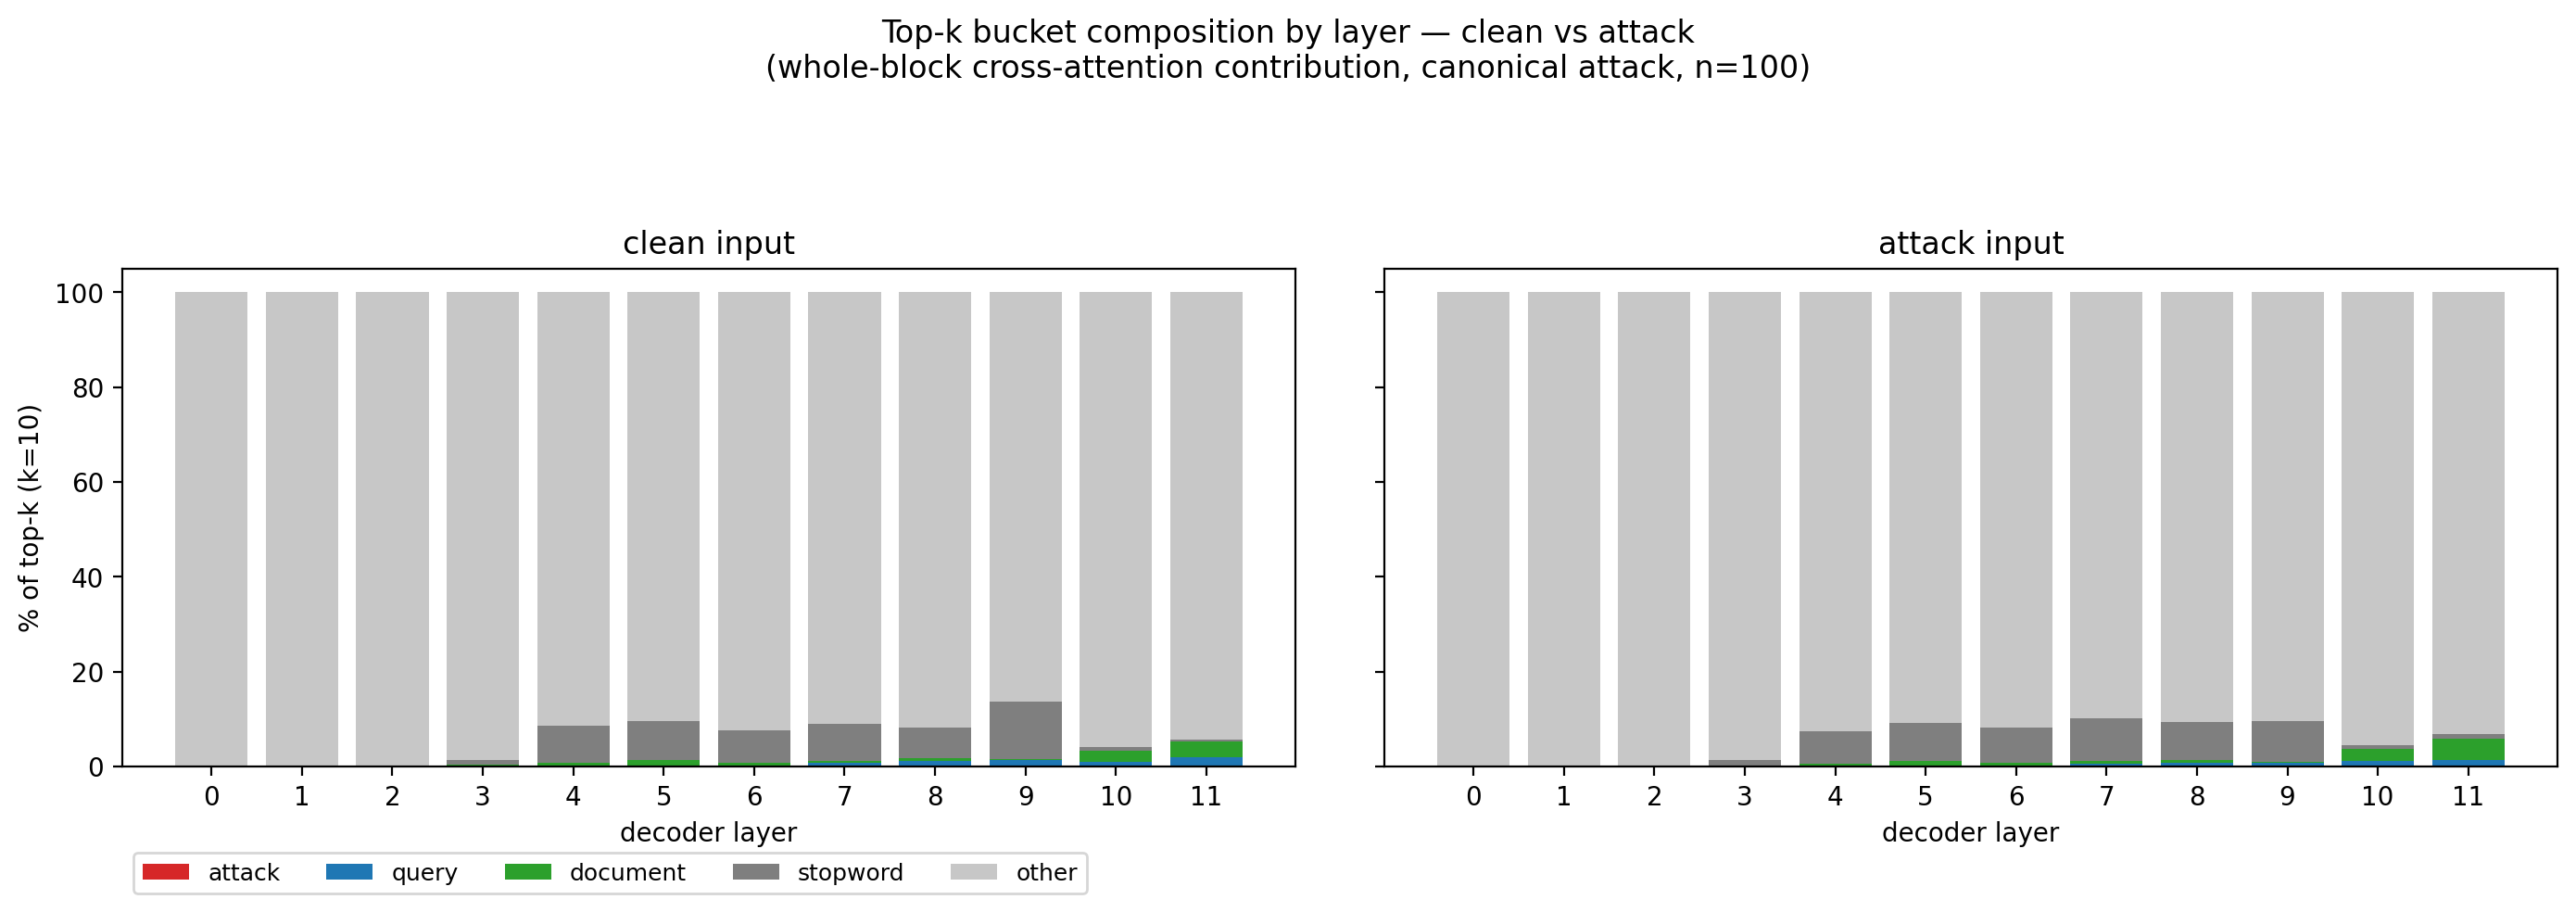
\includegraphics[width=0.95\textwidth]{outputs/plots/bucket_composition_by_layer.png}
  \caption{Top-10 bucket composition per decoder layer, clean vs.\ attack
  input, whole-block cross-attention contribution, canonical attack
  ($n=100$).}
  \label{fig:composition}
\end{figure}

The \texttt{attack} bucket is exactly $0.0\%$ of top-10 at \textbf{every
single layer, in both clean and attack runs}. \texttt{query} and
\texttt{document} together never exceed $\approx$5.8\% (layer~11, attack
run: query~$1.4\%$ + document~$4.4\%$); \texttt{other} is never below
$89\%$. The attack run and clean run's composition profiles are visually
almost indistinguishable (Figure~\ref{fig:composition}) — there is no
layer at which stuffing the document with the attack token causes that
token, or attack-adjacent vocabulary generally, to dominate the projected
top-10.

\subsection{The top tokens themselves are frequently uninterpretable}

Inspecting the actual most-frequent top-5 tokens (across the 100
canonical-attack examples) at individual flagged heads surfaces tokens with
no evident relationship to the query, document, or attack vocabulary — e.g.\
at layer~11, head~0: \texttt{stall, bleed, odonti[a], clove, pulp} (a
dental-medical cluster, unrelated to the DL19 query/document content or to
the word ``relevant''); at layer~11, head~2: \texttt{</s>, zahar
[Romanian: sugar], counter, man, hull}. These look like artefacts of
projecting an isolated, un-renormalised contribution vector through
\texttt{lm\_head} — the direction that vector points in vocabulary space
need not correspond to anything the model is ``about to say'' in the full
computation (Section~\ref{sec:discussion}).

\subsection{Per-head logit lens vs.\ whole-block}

\begin{figure}[H]
  \centering
  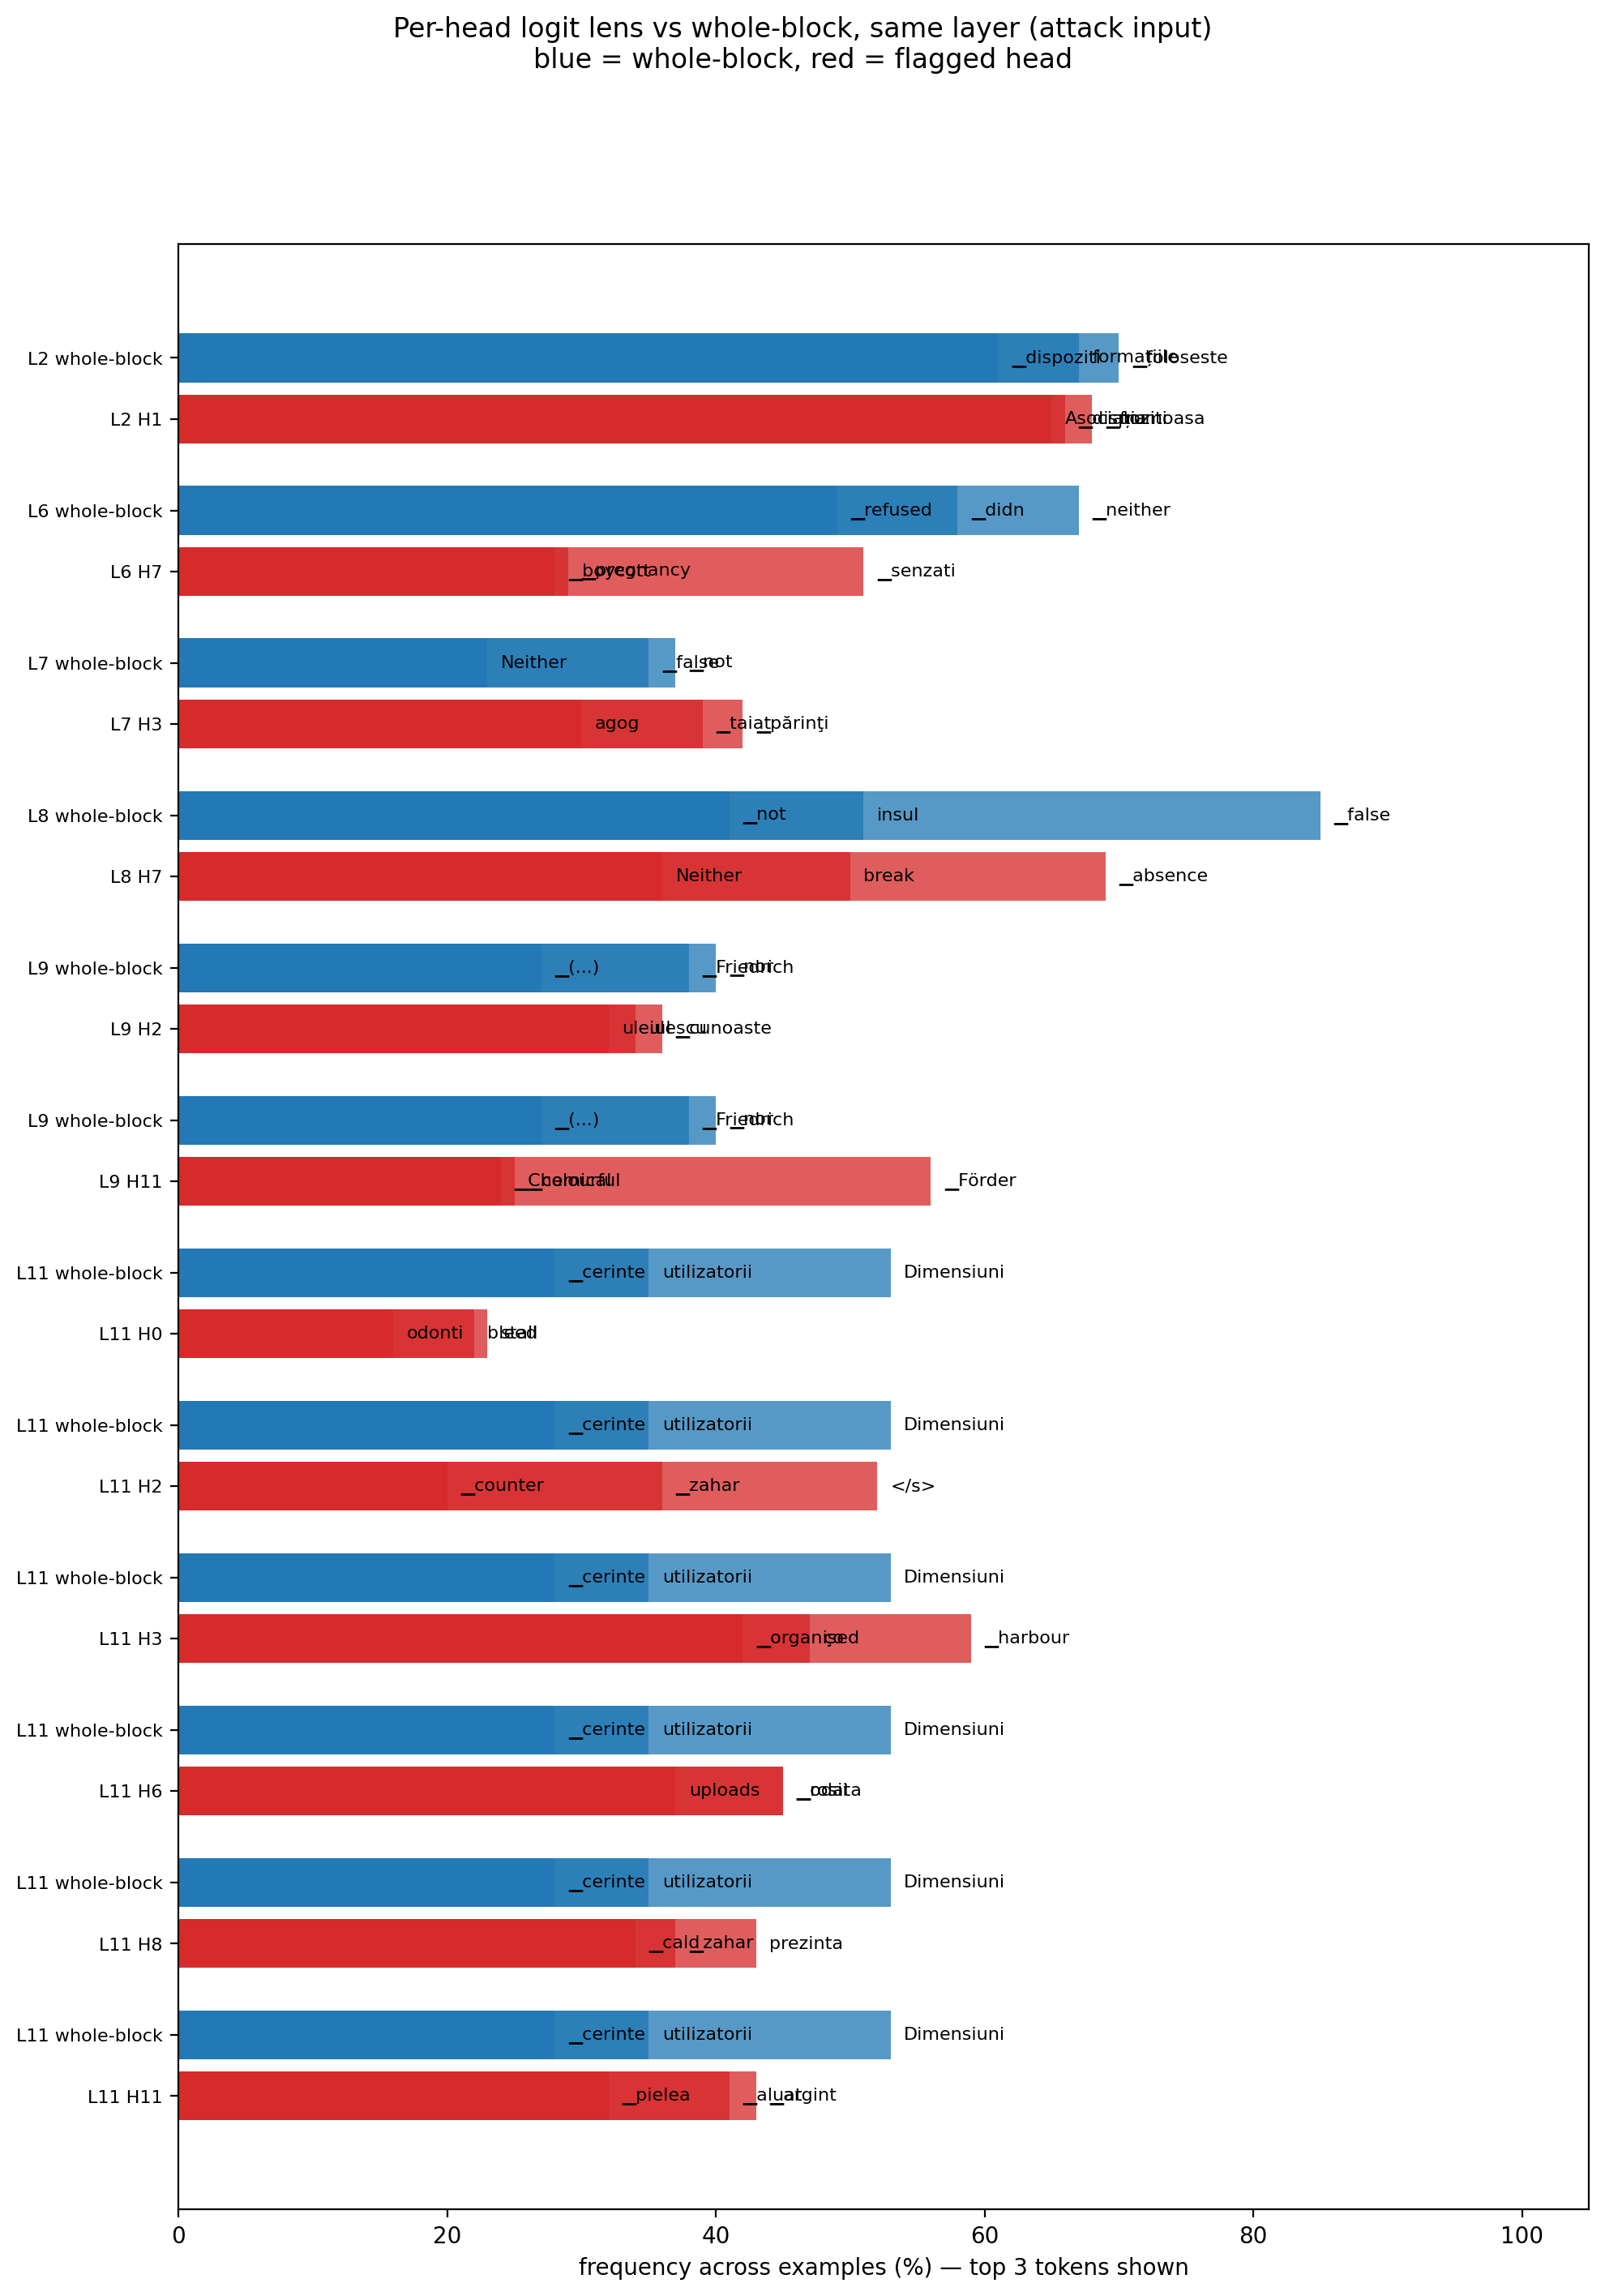
\includegraphics[width=0.95\textwidth]{outputs/plots/per_head_vs_whole_block.png}
  \caption{Most frequent top-5 tokens, flagged heads vs.\ whole-block, same
  layer, attack run (canonical attack, $n=100$).}
  \label{fig:perhead}
\end{figure}

No flagged head's top tokens are visibly more coherent or more
attack/query/document-relevant than the whole-block result at the same
layer — consistent with the attack-token-rank finding above (best per-head
rank, $6{,}472$, is worse than the whole-block's best, $8{,}741$ is
actually the whole-block number at L11 — per-head does not recover a
signal the whole-block sum is hiding).

% =====================================================================
\section{Discussion: why a null result here is not a contradiction of Experiments 1, 3, 6}
\label{sec:discussion}
% =====================================================================

\begin{enumerate}
  \item \textbf{Causal effect and direct logit attribution measure
  different things.} Experiments~1 and 3 show that \emph{patching}
  cross-attention's contribution at a given layer materially changes the
  final score — but that effect is realised by every subsequent layer
  processing the patched value, including possibly nonlinear
  transformations, further attention mixing, and the final
  \texttt{final\_layer\_norm} before read-out. A component can be causally
  important for the final answer without its own raw output, read in
  isolation, pointing anywhere near the relevant vocabulary direction —
  its job may be to shift what \emph{later} layers compute, not to
  directly encode the answer itself.
  \item \textbf{Skipping \texttt{final\_layer\_norm} is the most likely
  proximate cause of the uninterpretable top-$k$.} \texttt{lm\_head}'s
  weights were learned assuming their input has passed through
  \texttt{final\_layer\_norm}'s learned per-dimension rescaling. An
  isolated contribution vector, never rescaled that way, can have a very
  different effective magnitude profile across dimensions than what
  \texttt{lm\_head} expects, and the resulting projection can be dominated
  by whichever raw dimensions happen to be large — largely decoupled from
  the vector's actual semantic content. This was a deliberate, documented
  design choice (\texttt{DECISIONS.md}), following the direct-logit-
  attribution convention of not renormalising an isolated component — but
  the convention's known cost is exactly the kind of uninterpretable output
  observed here.
  \item \textbf{This experiment's own scope note anticipated this
  outcome.} \texttt{DECISIONS.md} states cross-attention-only scope should
  be revisited ``if cross-attention's logit-lens results are ambiguous or
  inconclusive.'' A clean $0\%$ attack-bucket rate and ranks in the tens of
  thousands are not ambiguous — they are a clear null result for this
  specific projection — but they do motivate the two follow-ups in
  Section~\ref{sec:limits}.
\end{enumerate}

\textbf{What this does \emph{not} do:} it does not cast doubt on
Experiments~1, 3, or 6's causal findings, which are established by patching
and ablation, a fundamentally different (interventional, not
representational) methodology, on the same cross-attention components.

% =====================================================================
\section{Limitations and Threats to Validity}
\label{sec:limits}
% =====================================================================

\begin{itemize}
  \item \textbf{No \texttt{final\_layer\_norm} re-application.} As
  discussed above, this is the most likely reason top-$k$ is
  uninterpretable. A natural follow-up applies the model's learned
  \texttt{final\_layer\_norm} \emph{scale} (not recomputed from the
  isolated vector's own statistics) to see whether that alone restores
  interpretable top-$k$, before concluding the component genuinely carries
  no directly-readable signal.
  \item \textbf{Cross-attention only, one component at a time.} The
  classical logit lens on the \emph{full accumulated residual stream} at
  each layer (rather than one sublayer's isolated contribution) was not
  run; it would test whether the null result is specific to isolating
  cross-attention or holds for the whole residual stream too.
  \item \textbf{Flagged-head snapshot is the $n=10$ list, not
  Experiment~3's revised $n=100$ list.} See Section~2.1. Given the
  magnitude of the null result (ranks in the thousands regardless of
  layer or head), it is unlikely a larger flagged-head set changes the
  conclusion, but this was not verified directly.
  \item \textbf{Single model/dataset.} Results are for monoT5-base on
  DL19, matching the rest of this project.
\end{itemize}

% =====================================================================
\section{Reproducibility}
% =====================================================================

From \texttt{07\_monot5\_logit\_lens/}, with the \texttt{advseq2seq} conda
environment and Experiments~1 and 3's outputs present as sibling
directories:

\begin{lstlisting}
bash bash/run_tests.sh          # unit tests (real tokenizer + tiny random T5, CPU)
bash bash/run_pilot.sh          # timing pilot
bash bash/run_all.sh            # full pipeline (resume-safe)
\end{lstlisting}

\noindent On this run: SLURM job on 1$\times$ L40 GPU, $\approx$1~hour~
10~minutes wall-clock for both runs plus aggregation and plotting; outputs
under \texttt{outputs/\{grid,canonical\}/} and \texttt{outputs/plots/}.

% =====================================================================
\section*{Appendix: Glossary of Key Quantities}
\addcontentsline{toc}{section}{Appendix: Glossary of Key Quantities}
% =====================================================================

\begin{description}[leftmargin=1.6em,style=nextline]
  \item[contribution] $\text{out\_hidden} - \text{in\_hidden}$ of a
  cross-attention sublayer — what it writes into the residual stream.
  \item[direct logit attribution] projecting an isolated component's
  contribution through the model's unembedding, without re-applying
  \texttt{final\_layer\_norm}; distinct from classical full-residual logit
  lens.
  \item[attack\_token\_rank / logit] the specific injected token's
  1-indexed rank (1 = top) and raw logit in this projection, tracked for
  clean, control, and attack inputs.
  \item[bucket composition] \% of top-$k$ tokens tagged attack / query /
  document / stopword / other.
  \item[whole-block / per-head] all 12 heads' summed contribution vs.\ one
  Experiment-3-flagged head's contribution alone ($W_o(\text{zero\_pad}
  (\cdot))$).
\end{description}

\end{document}
